\documentclass{cumcmthesis}
% \documentclass[withoutpreface,bwprint]{cumcmthesis} %去掉封面与编号页,电子版提交的时候使用。


\usepackage[framemethod=TikZ]{mdframed}
\usepackage{url}   % 网页链接
\usepackage{subcaption} % 子标题
\title{全国大学生数学建模竞赛编写的 \LaTeX{} 模板}
\tihao{A}
\baominghao{4321}
\schoolname{XX大学}
\membera{ }
\memberb{ }
\memberc{ }
\supervisor{ }%辅导老师
\yearinput{2023}
\monthinput{9}
\dayinput{8}

\begin{document}

 \maketitle
 \begin{abstract}%摘要在这里写

\keywords{\TeX{}\quad  图片\quad   表格\quad  公式}
\end{abstract}

%目录  2019 明确不要目录,我觉得这个规定太好了
%\tableofcontents

%\newpage

\section{问题重述}%1
\subsection{问题背景}
\subsection{问题提出}
\section{问题分析}%2
\section{模型假设与符号说明}%3
\subsection{模型假设}
\subsection{符号说明}
\section{问题一模型建立与求解}%4

\subsection{数据预处理}

\subsubsection{异常值处理}
在附件内容没有明显缺失的情况下, 数据中可能出现异常值. 对具体的单品而言, 考虑到季节变化, 天气影响和送货环节异常等情况, 加之2020—2023年期间新冠疫情的存在, 上述内容可能使得部分蔬菜销量受到一定影响, 它们所造成的局部异常值, 极端值对统计销量和蔬菜相互关系以及后续预测蔬菜需求不具有普适性意义. 因此, 需要预处理异常值, 将其转化为可观测范围内的正常, 或直接舍弃. 

依据附件1的''分类编码''字段, 将251个单品映射至六大品类 (花菜类、食用菌、花叶类、辣椒类、茄类、水生根茎类). 采用箱线图处理异常值, 记各类别蔬菜的下四分位点, 中位数和上四分位点为$Q_1$,$Q_2$,$Q_3$; 四分位距为$IQR=Q_3-Q_1$. 获取各单品蔬菜中超出正常分布区间的异常值, 异常值处理方法如下:

Step1 对附件2中全部''销量(千克)''字段按单品编码分别提取并排序,计算第一四分位数$Q_1$与第三四分位数$Q_3$, 得到四分位距 $IQR_{1-3}=Q_3-Q_1$。

Step2 稳健区间为
\[ [Q_1 - 1.5 \cdot IQR, Q_3 + 1.5 \cdot IQR] \]
落在区间外的观测记为异常. 对异常值进一步区分: 
若异常发生于春节, 中秋和疫情封控等已知事件对应日期, 视为''可解释异常'', 予以保留;其余异常视为''极端噪声'', 用该单品前后各3天正常销量的中位数进行替换, 以保证时间序列的连续性与季节性特征不被破坏.  

Step3 将修正后的数据按日期重新对齐, 确保每条记录均包含单品编码, 销售日期和销量 (千克)三列, 形成异常值已清洗的原始库. 

以花菜类蔬菜为例, 三年总销量的日销量为纵轴, 星期属性为横轴, 绘制箱型图如下: 
\begin{figure}[H]
    \centering
    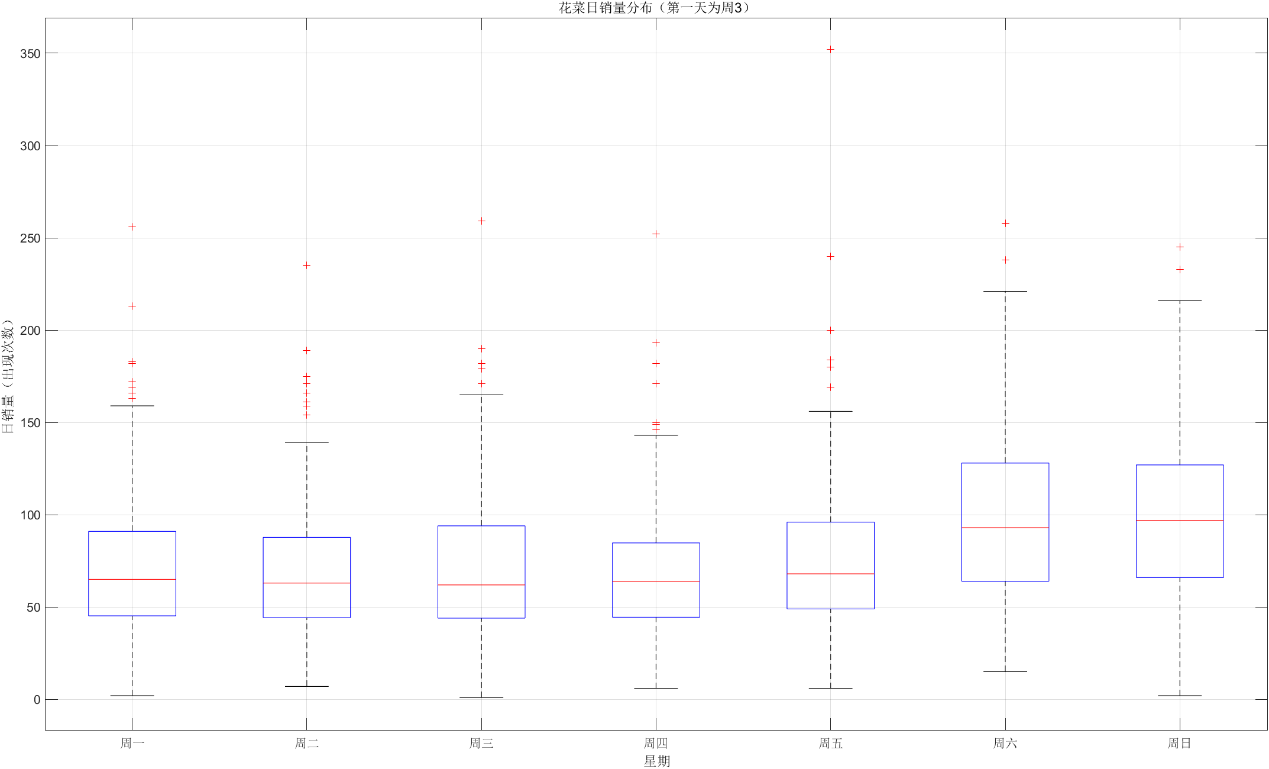
\includegraphics[width=0.8\textwidth]{花菜日销量分布(第一天为周3).png} 
    \caption{花菜类蔬菜日销量分布箱型图(第一天为周三)}
\end{figure}


\subsubsection{数据清洗整合}

以“品类编码+销售日期”为键, 对清洗后的销量进行汇总, 得到六大品类的日销量序列; 随后以7天为窗口滑动求和, 生成周销量序列;以自然月为周期求和, 生成月销量序列。  

兼顾精细化需求, 按小时、日、周、月四种粒度分别构建以下矩阵: 

(1)小时级: 提取原始流水中的''销售时间''字段, 汇总至 0-23 点, 形成24品类矩阵, 用于日内波动分析; 

(2)日级: 每日品类销量矩阵, 覆盖2020-07-01至2023-06-30共1095 d;   

(3)周级: 按ISO 周历汇总, 共157周;   

(4)月级: 按自然月汇总, 共36个月. 

最后, 将上述矩阵统一存储为''时间$\times$品类''的二维表, 缺失值用0填充, 形成后续ARIMA建模, 相关性分析与聚类分析的标准输入. 

\subsection{销售量的分布规律}

\subsubsection{多时间粒度的类间销售量比较}
\begin{figure}[H]
    \centering
    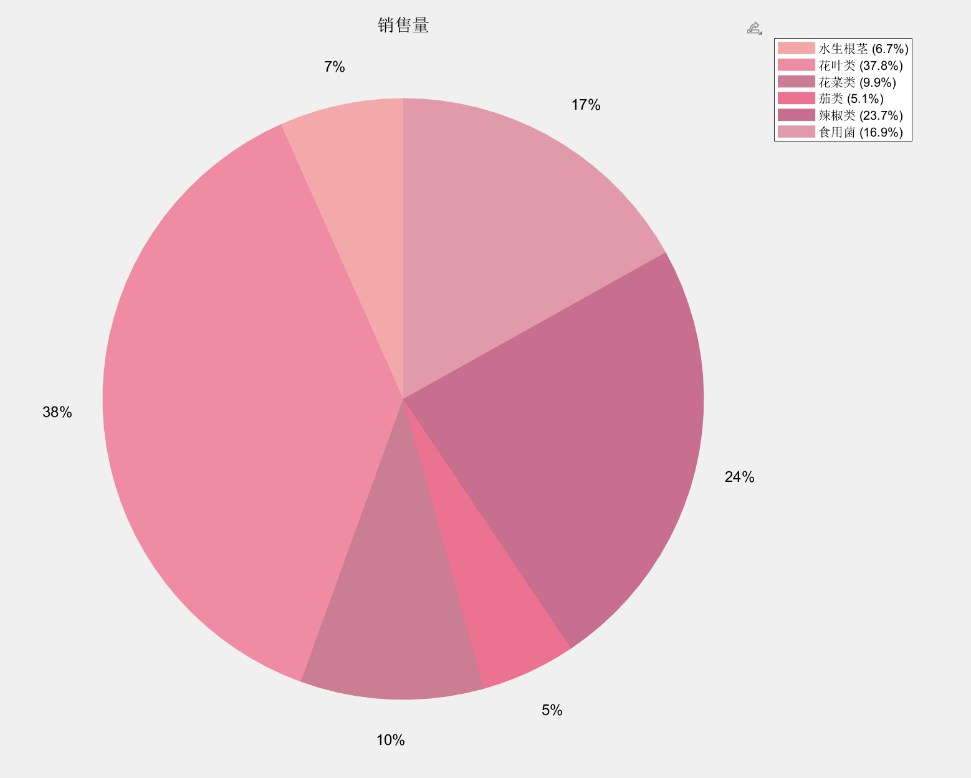
\includegraphics[width=0.6\textwidth]{销售量占比.png} 
    \caption{六大品类蔬菜销售量占比图}
\end{figure}

在清洗后的数据基础上, 统计六大类别的蔬菜销售量占比. 花叶类总销量位于所有蔬菜品类销量之首, 占比达到37.8%;辣椒类和食用菌类的蔬菜占比分别达到23.7%和16.9%;花菜类、水生根茎类和茄类的总销量占比较少。花叶类蔬菜是数据量最庞大、最具有代表性的对象,下述的统计数据与模型建立主要以花菜类蔬菜为例加以说明,其余从略。

我们还需要得出具体的, 各品类的销售情况与相互关系. 由于附件所给数据为时间序列数据,因此必须考虑时间效应,兼顾精细化需求,按月、日、小时不同的时间粒度,绘制时间序列图。

花叶蔬菜的三年总销量的日销量逐日分布折线比较图如下, 尽管2022年1月前后的日销量水平与2021年、2023年同期水平相比较低, 该图仍然反映了一定的时间依赖性, 如: 花叶类蔬菜日销售量1月左右销量步入低潮、6月后逐步销量步入升高。这与花叶类蔬菜本身的季节性、周期性有关。此外,在销售中,总是出现“锯齿状”的图样,通过映射比较附件2中的日期数据,发现节假日期间日销量会抬升,周末总销量高于工作日,反映出顾客集中采购行为增加;工作日销量平稳,各品类占比稳定。总之,该图像反应花叶类销售呈现明显的时间依赖性,适合构建单变量时间序列。

\begin{figure}[H]
    \centering
    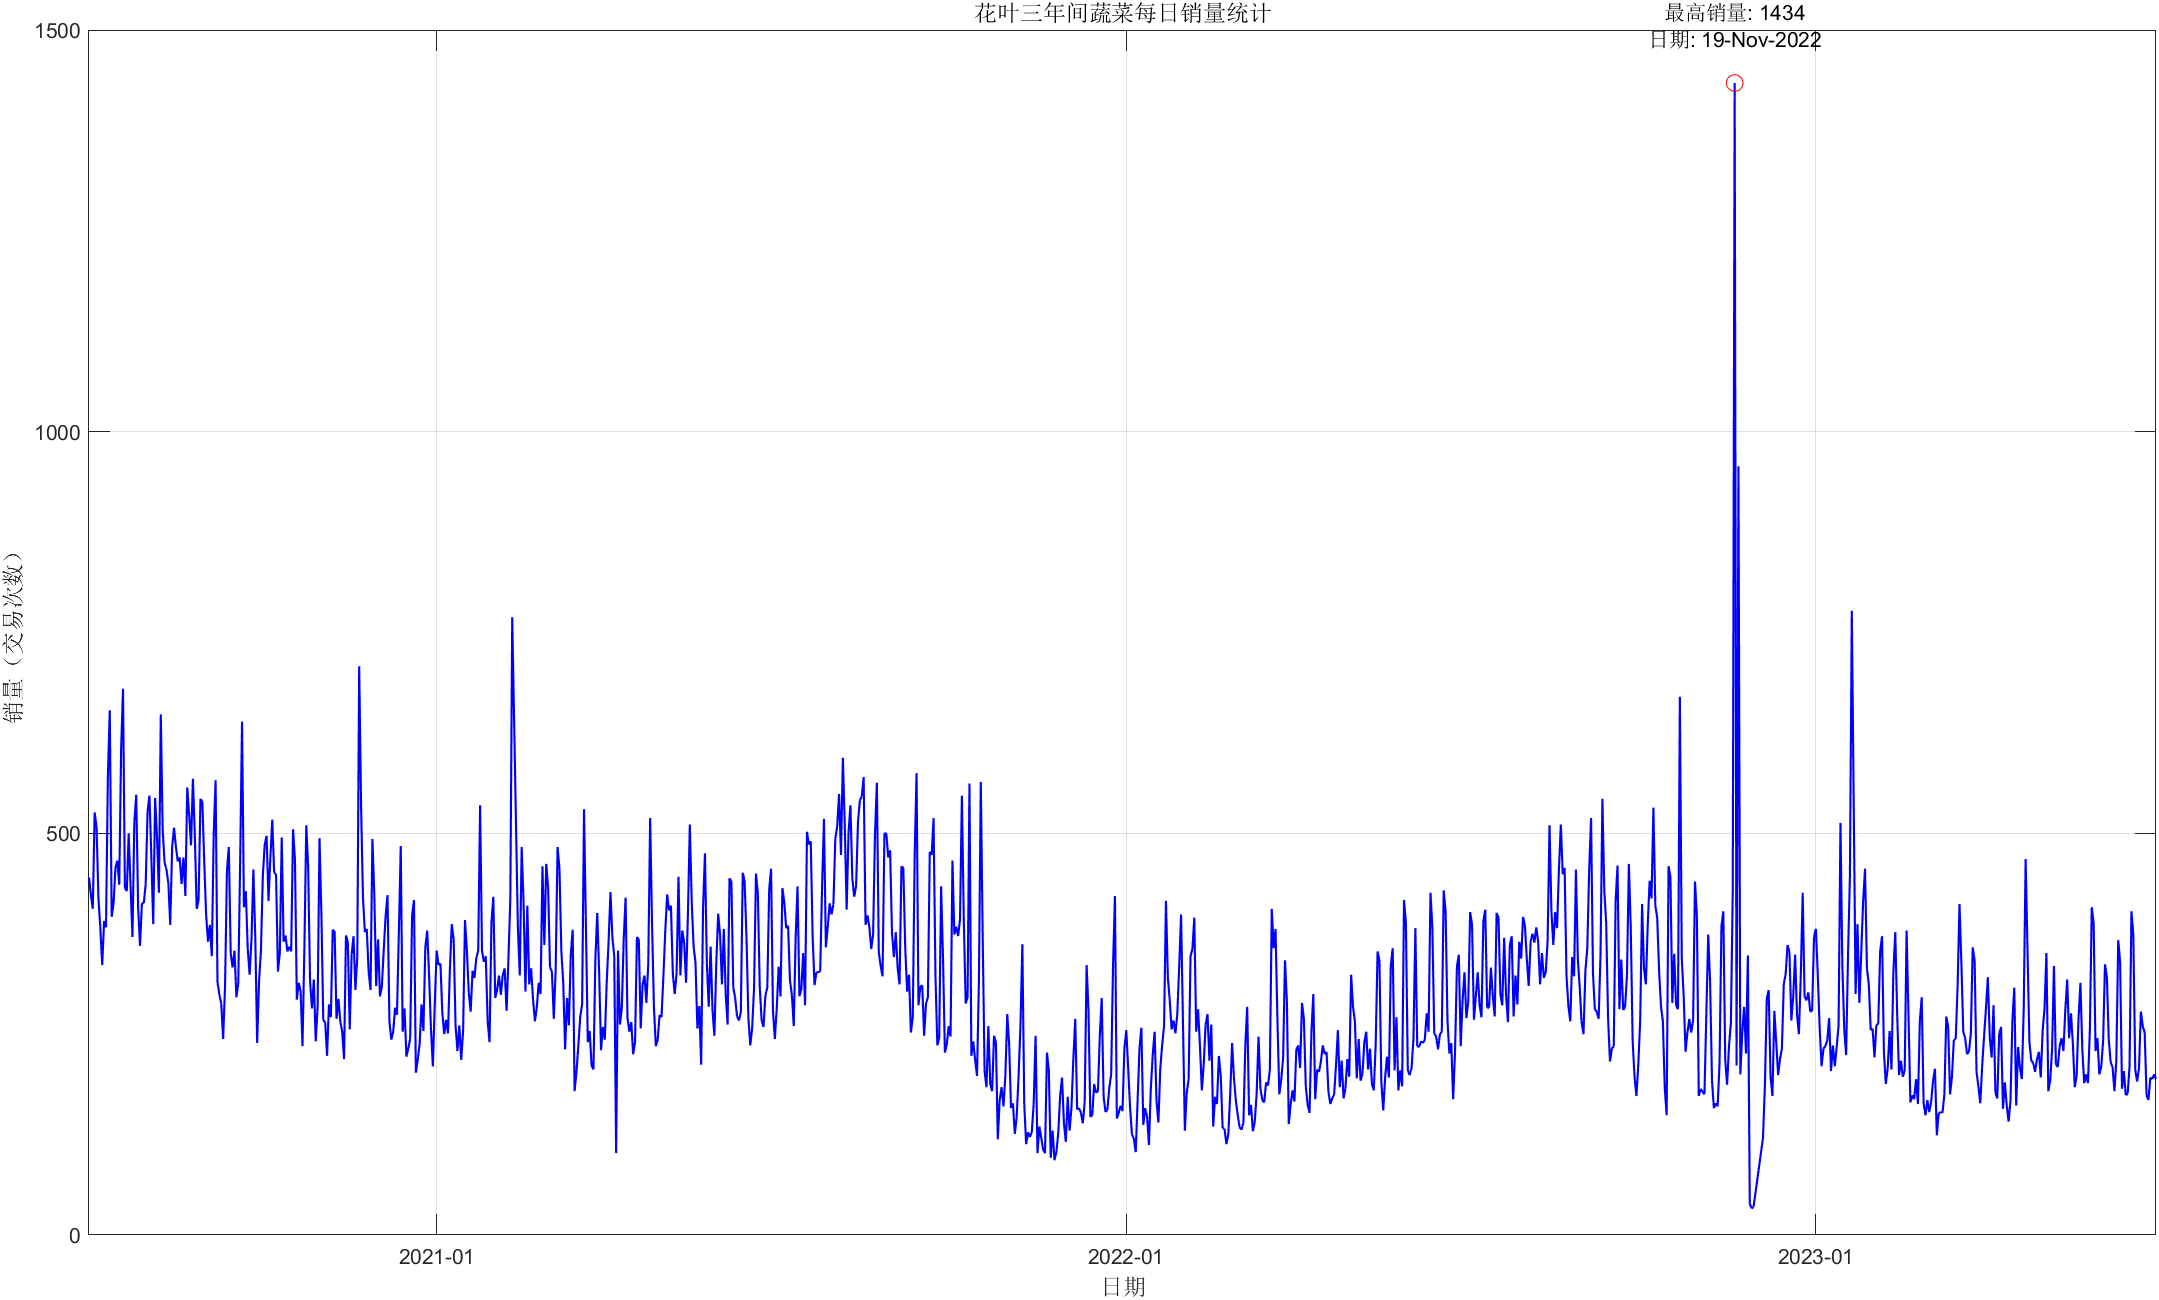
\includegraphics[width=0.8\textwidth]{花叶三年间蔬菜每日销量统计.png} 
    \caption{花叶类蔬菜三年每日销量统计折线图}
\end{figure}

\begin{figure}[H]
    \centering
    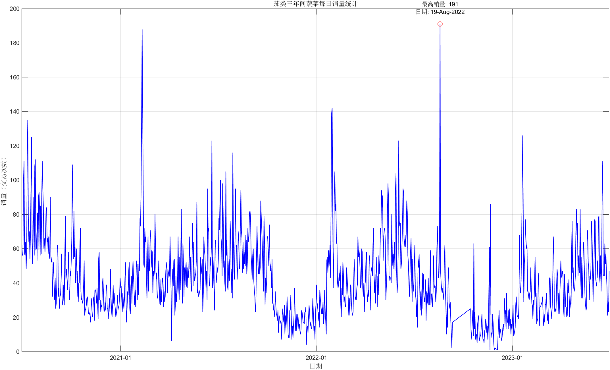
\includegraphics[width=0.8\textwidth]{其他品类日销量折线图1.png} 
    \caption{部分品类蔬菜三年每日销量统计折线图(一)}
\end{figure}

\begin{figure}[H]
    \centering
    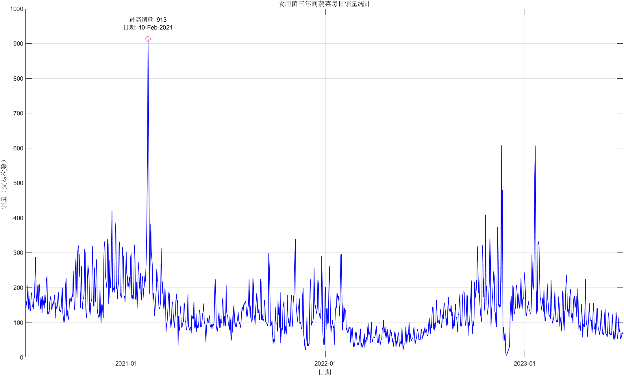
\includegraphics[width=0.8\textwidth]{其他品类日销量折线图2.png} 
    \caption{部分品类蔬菜三年每日销量统计折线图(二)}
\end{figure}

\begin{figure}[H]
    \centering
    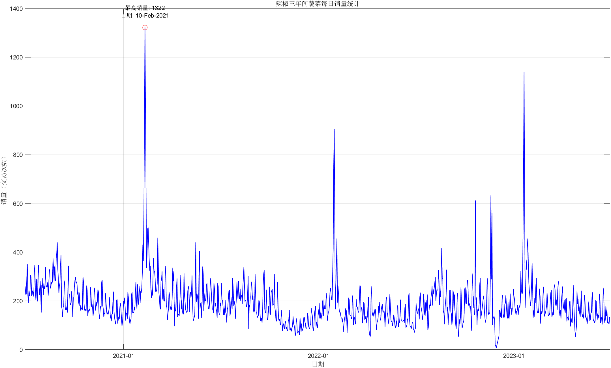
\includegraphics[width=0.8\textwidth]{其他品类日销量折线图3.png} 
    \caption{部分品类蔬菜三年每日销量统计折线图(三)}
\end{figure}

为了验证、推广上述分析, 其他类别蔬菜的缩略图如下. 茄类、水生根茎、辣椒类、食用菌类蔬菜的三年总销量的日销量逐日分布折线比较图如上. 从图中可以看出, 其峰值节点、日销售量趋势变化均呈现规律排布. 蔬菜品类的日销量具有显著的时间依赖性, 构成单变量时间序列, 并表现出明显的季节性、周期性和节假日效应. 而且, 长期来看各个品类销售占比较为稳定, 因此, 可针对各品类的日销量序列, 采用时间序列建模方法对其变动趋势进行模拟与预测.

\begin{figure}[H]
    \centering
    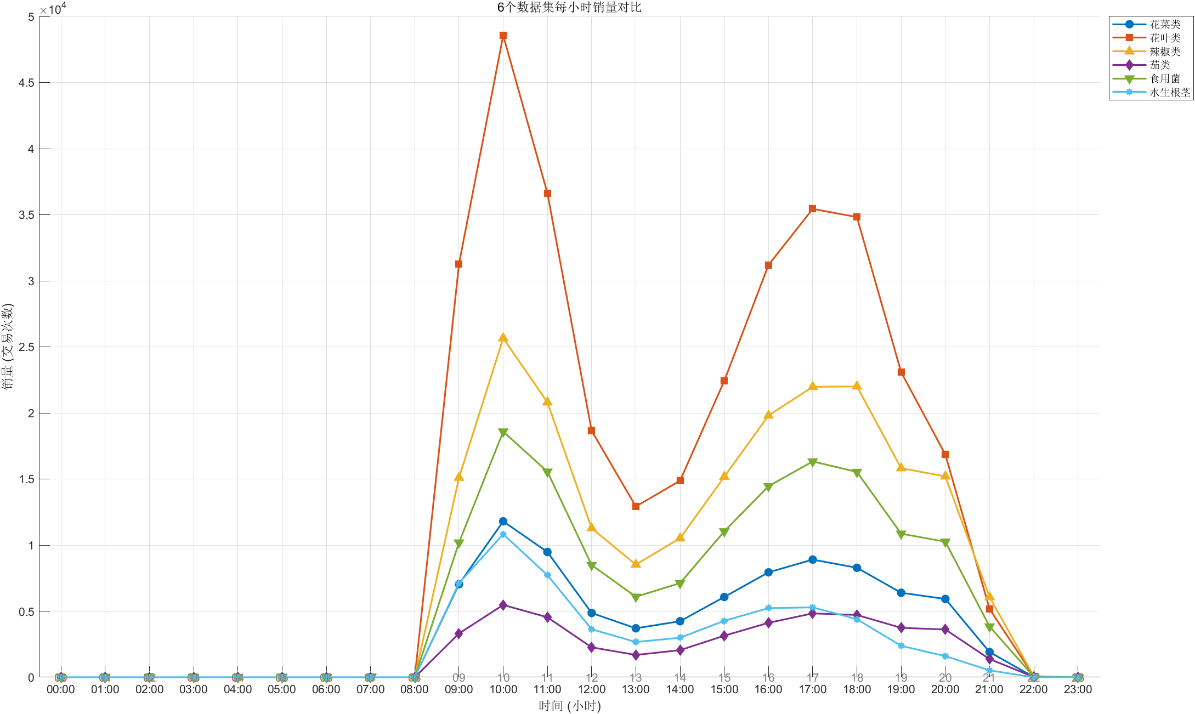
\includegraphics[width=0.8\textwidth]{6个数据集每小时销量对比.png} 
    \caption{六类蔬菜每小时销量对比图}
\end{figure}

六类蔬菜的三年总销量的平均日销量逐小时分布折线比较图如上. 花叶类蔬菜从早上8点至晚上10点持续有销量、且销售量折线基本覆盖其他类别蔬菜, 说明该类蔬菜是民众三餐常备菜品. 整体来看, 所有菜品的销量在上午10点和下午17点达到峰值, 恰好对应于午餐和晚餐前的备菜高峰, 符合现实情况.

\subsubsection{ARIMA 时间序列分析设计}

\paragraph{时间序列建模}
ARIMA (自回归积分移动平均模型) 是时间序列分析中常用的预测模型, 适于处理非平稳时间序列数据. 

ARIMA模型由三部分组成, 记为ARIMA(p,d,q), 其中: 


(1) AR(p)自回归: 利用序列自身的滞后项(过去值)预测当前值, p为滞后项数。例如, p=2表示用前2期的值预测当前值. 

(2) I(d)积分: 通过对非平稳序列进行d次差分, 使其转化为平稳序列, d为差分次数 (通常d=0,1,2). 

(3) MA(q)移动平均: 关注自回归模型中误差项的累计, 利用序列的滞后误差项(预测误差)修正当前预测, q为误差项的滞后项数. 

根据需求分析维度, 建立以周为时间粒度的销量序列, 以捕捉周内需求波动、周度工作日—周末差异及季节性产地转换效应。  

建模流程如下:  


Step1 检查时间序列的连续性、绘制时序图  

Step2 平稳性检验, 若时序图显示非平稳 (有明显趋势), 需通过差分法通过ADF检验 (单位根检验)  

Step3 基于平稳后的序列, 绘制ACF (自相关函数)图和PACF (偏自相关函数)图  

\begin{figure}[H]
    \centering
    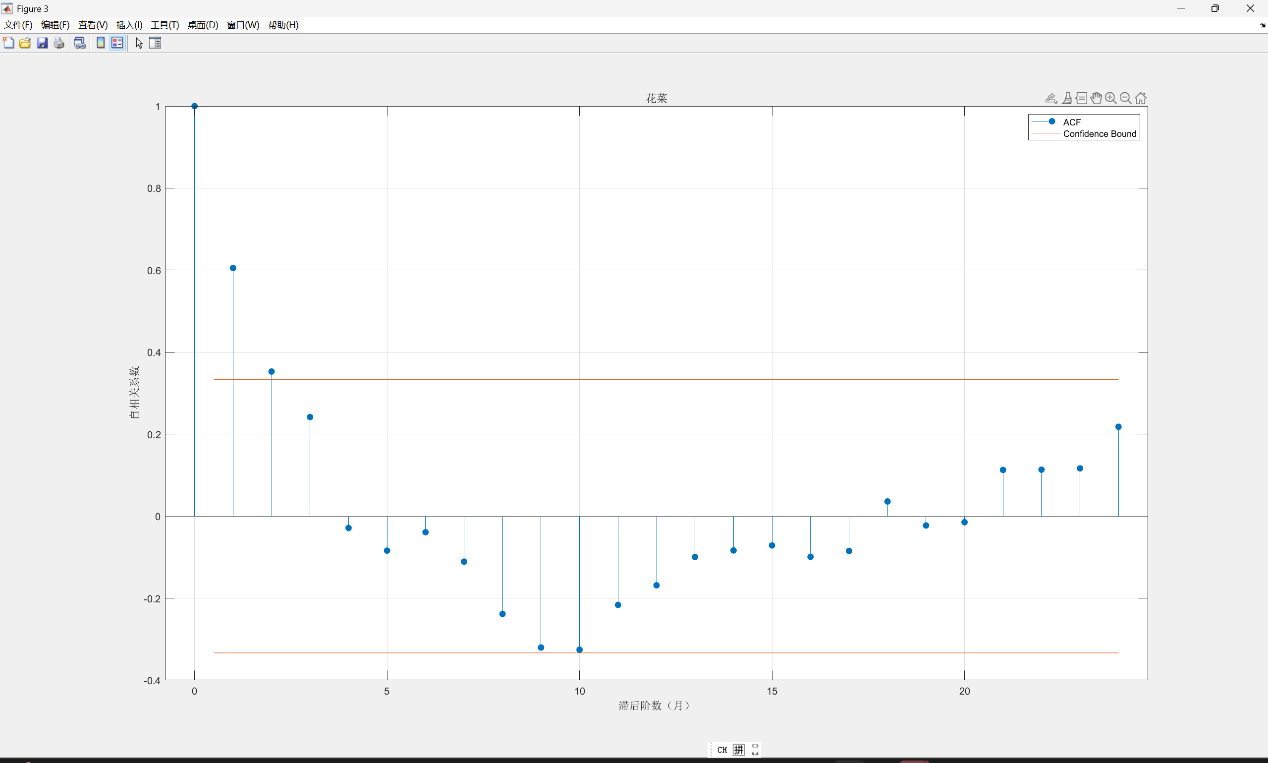
\includegraphics[width=0.8\textwidth]{花菜ACF图.png} 
    \caption{花菜类蔬菜销量ACF图 (滞后阶数:周)}
\end{figure}

\subsection{销售量的相互关系}

\subsubsection{品类间的Pearson和Spearman相关系数分析}
为分析六大蔬菜品类 (花叶类、花菜类、水生根茎类、茄类、辣椒类、食用菌)间的相互关系, 结合Pearson相关系数和Spearman等级相关系数, 从线性和单调两个维度量化品类间的关联性, 以识别互补或替代关系. 

\subsubsection{方法原理与适用性}
1. \textbf{Pearson相关系数}:   
核心原理基于协方差与标准差,衡量连续变量间的线性相关程度,公式为:  
\begin{equation}
r=\frac{Cov(X,Y)}{\sigma_x \cdot \sigma_y}
\end{equation}  

其中$Cov(X,Y)$为协方差,$\sigma_x$和$\sigma_y$分别为变量$X$和$Y$的标准差.  

适用场景: 变量为连续型, 数据近似服从正态分布或样本量$n>30$, 且关系呈线性 (点图呈直线趋势). 

局限性: 对异常值敏感, 需通过数据预处理剔除极端值. 

2. \textbf{Spearman等级相关系数}:   
核心原理基于秩次转换, 将数据按大小排序为等级, 衡量单调关系 (同增或同减趋势), 公式为: 
\begin{equation}
\rho=1-\frac{6\sum d_i^2}{n(n^2-1)}
\end{equation}  
其中$d_i$为两变量秩次差,$n$为样本量.  
适用场景: 变量为连续型或有序分类 (如销量等级), 关系单调但非线性, 数据非正态或含异常值时更稳健.

\subsubsection{分析流程设计}
\begin{enumerate}
    \item 数据预处理: 聚合品类日销量数据, 缺失值以0填充 (无销售日), 异常值通过四分位距 (IQR)法处理 (替换为均值); 标准化销量以消除量纲影响. 
    \item 相关系数计算与检验: 分别计算日销量和月销量的Pearson $r$与Spearman $\rho$。日销量反映短期波动关系 (如节假日前替代效应); 月销量平滑噪声, 捕捉季节性趋势. 
    \item 显著性检验: 通过$t$-检验 ($t=\frac{r(n-2)}{\sqrt{1-r^2}}$,自由度$df=n-2$)验证相关性,$P<0.05$视为显著相关 (非随机误差). 
    \item 关系解读规则: 
    (1)替代关系:显著负相关 ($r<0$或$\rho<0$, $p<0.05$), 如辣椒类与花叶类竞争消费者预算; 

    (2)互补关系:显著正相关 ($r>0$或$\rho>0$, $p<0.05$), 如花菜类与食用菌常搭配销售;  

    (3)无关性:$|r|$或$|\rho|$接近0或$p≥0.05$.

    可视化辅助:通过相关系数矩阵热力图直观展示品类关联强度与方向. 
\end{enumerate}

\subsubsection{相关系数矩阵} 
\paragraph{Pearson相关系数矩阵}
\begin{table}[H]
\centering
\begin{tabular}{c c c c c c c}
\toprule
品类 & 水生根茎 & 花叶类 & 花菜类 & 茄类 & 辣椒类 & 食用菌 \\
\midrule
水生根茎 & / & 0.42 & 0.38 & -0.15 & 0.38 & 0.62 \\
花叶类 & / & / & 0.60 & 0.37 & 0.66 & 0.61 \\
花菜类 & / & / & / & 0.22 & 0.48 & 0.49 \\
茄类 & / & / & / & / & 0.22 & -0.01 \\
辣椒类 & / & / & / & / & / & 0.57 \\
食用菌 & / & / & / & / & / & / \\
\bottomrule
\end{tabular}
\end{table}

\paragraph{Spearman相关系数矩阵}
\begin{table}[H]
\centering
\begin{tabular}{c c c c c c c}
\toprule
品类 & 水生根茎 & 花叶类 & 花菜类 & 茄类 & 辣椒类 & 食用菌 \\
\midrule
水生根茎 & / & 0.42 & 0.39 & -0.19 & 0.33 & 0.61 \\
花叶类 & / & / & 0.63 & 0.32 & 0.59 & 0.60 \\
花菜类 & / & / & / & 0.24 & 0.43 & 0.46 \\
茄类 & / & / & / & / & 0.16 & -0.09 \\
辣椒类 & / & / & / & / & / & 0.53 \\
食用菌 & / & / & / & / & / & / \\
\bottomrule
\end{tabular}
\end{table}


\subsection{单品聚类分析:群体特征与关系分组}
\subsubsection{方法原理与优势}

1. \textbf{核心原理}: 采用K-means聚类算法, 通过最小化簇内平方误差 (SSE) 划分单品, 公式为: 
\begin{equation}
SSE=\sum_{i=1}^{K}\sum_{x\in C_i}||x-\mu_i||^2
\end{equation}  
其中$\mu_i$为第$i$个簇的质心,$x$为数据点,欧氏距离度量相似性:  
\begin{equation}
d(x,y)=\sqrt{\sum (x_i-y_i)^2}
\end{equation}

2. \textbf{优势}: 可处理高维数据 (如单品销量、价格、季节性指标), 通过分组降低复杂度, 识别隐性关联 (如“时令蔬菜群”). 
3. \textbf{补充作用}: 弥补相关系数仅限两两关系的局限性, 揭示全局结构 (如“替代品群组”). 

\subsubsection{分析流程设计}

\begin{enumerate}
    \item 特征工程: 提取单品特征 (月销量比例、年销量趋势、价格弹性), 标准化特征以避免量纲偏差. 
    \item 聚类步骤: 
    (1)确定$K$值: 根据业务需求(如商超品类管理目标)或肘部法;

    (2)初始化质心: 采用$K-means++$算法优化,确保质心分散; 

    (3)迭代优化:分配数据点 (计算单品到各质心的欧氏距离, 归入最近簇), 更新质心(重算簇内均值作为新质心),直至质心变化$<\epsilon$或达最大迭代次数. 
    
    \item 群体关系解析: 
    (1)组内关系: 高相似单品可能互补,如“叶菜群”中菠菜、油麦菜需求同增; 

    (2)组间关系: 不同群可能替代,如“茄果群”与“根茎群”竞争货架空间; 

    (3)异常组: 独立群(如珍稀食用菌),与其他品类需求无关. 
    \item 可视化输出: 通过聚类热力图叠加相关系数展示关系 (如组内强正相关、组间强负相关). 
\end{enumerate}

\subsubsection{聚类结果 (针对销量显著的30个单品)}

\begin{figure}[H]
    \centering
    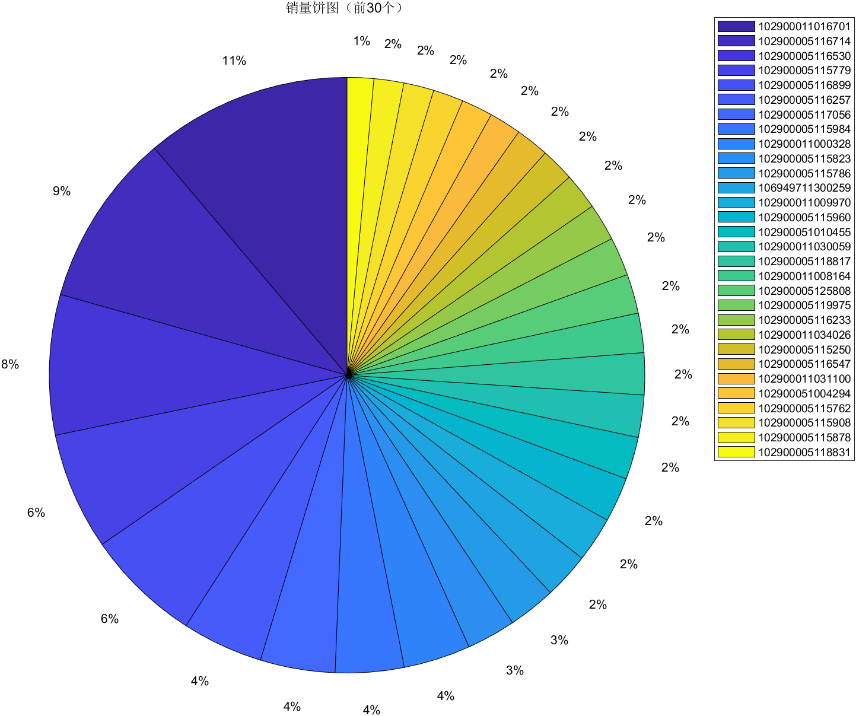
\includegraphics[width=0.7\textwidth]{销量饼图(前30个).png} 
    \caption{前30个高销量单品销量占比饼图}
\end{figure}

\begin{figure}[H]
    \centering
    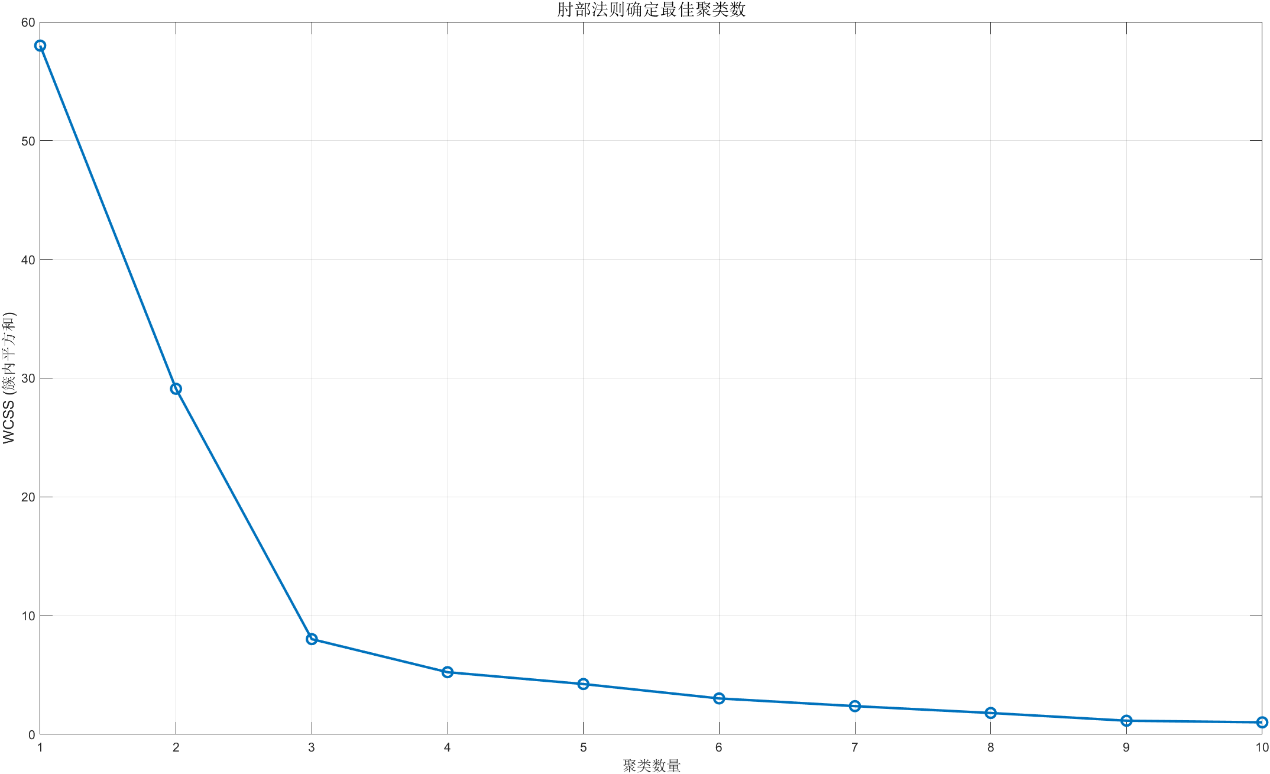
\includegraphics[width=0.7\textwidth]{聚类肘部图.png}
\end{figure}

\begin{figure}[H]
    \centering
    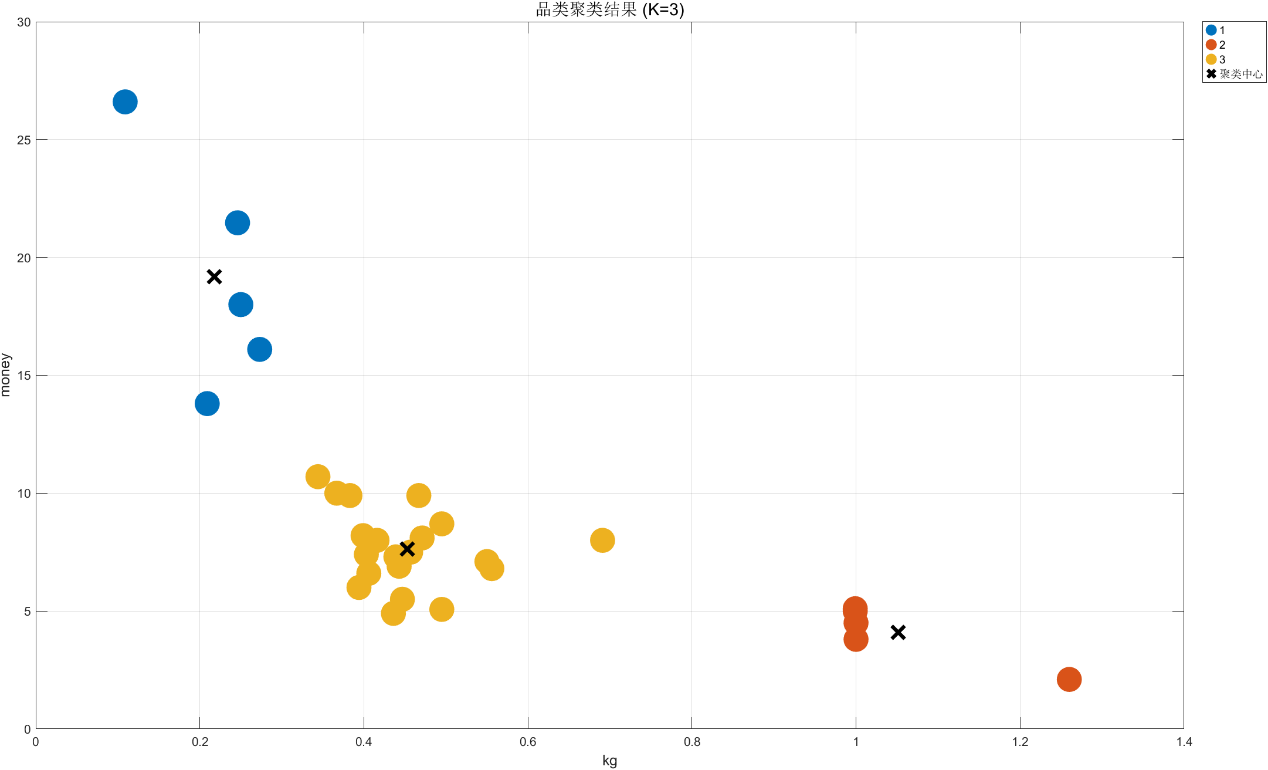
\includegraphics[width=0.7\textwidth]{聚类结果可视化.png}
    \caption{单品聚类结果可视化图}
\end{figure}

聚类评价指标结果:
\begin{figure}[H]
    \centering
    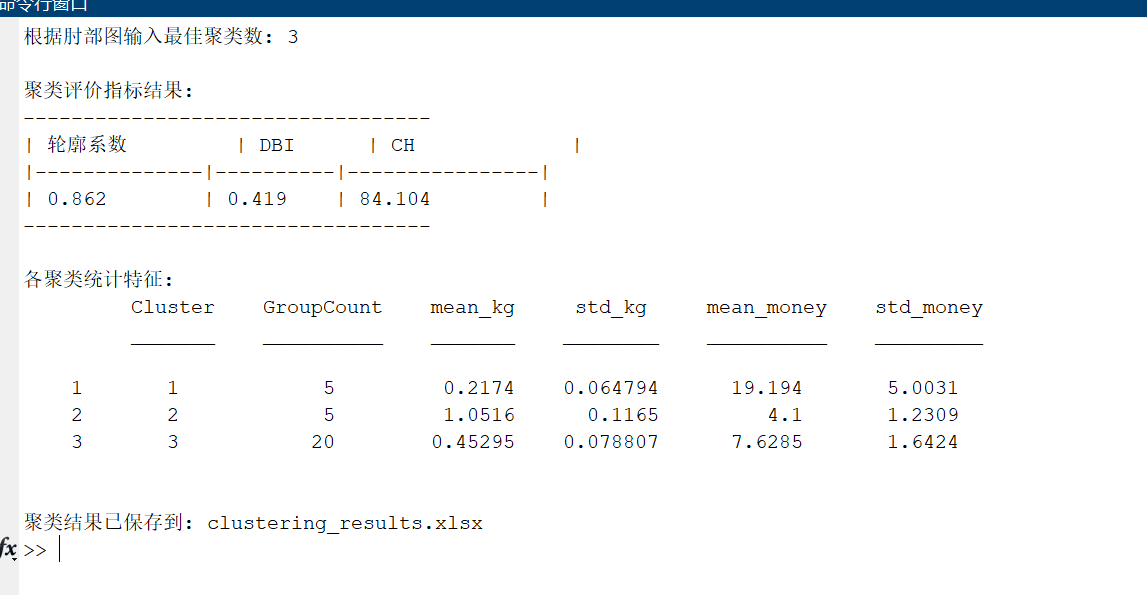
\includegraphics[width=0.7\textwidth]{结果.png}
    \caption{结果图}
\end{figure}

\begin{table}[H]
    \centering
    \begin{tabular}{c c c}
    \toprule
    轮廓系数 & DBI & CH \\
    \midrule
    0.862 & 0.419 & 84.104 \\
    \bottomrule
    \end{tabular}
\end{table}

各聚类统计特征:
\begin{table}[H]
    \centering
    \begin{tabular}{c c c c c}
    \toprule
    Cluster & GroupCount & mean\_kg & mean\_money & std\_money \\
    \midrule
    1 & 5 & 1.0516 & 1.2309 & 4.1 \\
    2 & 20 & 0.45295 & 7.6285 & 1.6424 \\
    3 & 1 & 0.2174 & 19.194 & 5.0031 \\
    \bottomrule
    \end{tabular}
\end{table}

%参考文献
\begin{thebibliography}{9}%宽度9
    \bibitem[1]{liuhaiyang2013latex}
    刘海洋.
    \newblock \LaTeX {}入门\allowbreak[J].
    \newblock 电子工业出版社, 北京, 2013.
    \bibitem[2]{mathematical-modeling}
    全国大学生数学建模竞赛论文格式规范 (2023 年 修改).
    \bibitem{3} \url{https://www.latexstudio.net}
\end{thebibliography}

\newpage
%附录
\begin{appendices}

\section{模板所用的宏包}
\begin{table}[htbp]
    \centering
    \caption{宏包罗列}
    \begin{tabular}{ccccc}
        \toprule
        \multicolumn{5}{c}{模板中已经加载的宏包} \\
        \midrule
        amsbsy & amsfonts & {amsgen} & {amsmath} & {amsopn} \\
        amssymb & amstext & {appendix} & {array} & {atbegshi} \\
        atveryend & auxhook & {bigdelim} & {bigintcalc} & {bigstrut} \\
        bitset & bm    & {booktabs} & {calc} & {caption} \\
        caption3 & CJKfntef & {cprotect} & {ctex} & {ctexhook} \\
        ctexpatch & enumitem & {etexcmds} & {etoolbox} & {everysel} \\
        expl3 & fix-cm & {fontenc} & {fontspec} & {fontspec-xetex} \\
        geometry & gettitlestring & {graphics} & {graphicx} & {hobsub} \\
        hobsub-generic & hobsub-hyperref & {hopatch} & {hxetex} & {hycolor} \\
        hyperref & ifluatex & {ifpdf} & {ifthen} & {ifvtex} \\
        ifxetex & indentfirst & {infwarerr} & {intcalc} & {keyval} \\
        kvdefinekeys & kvoptions & {kvsetkeys} & {l3keys2e} & {letltxmacro} \\
        listings & longtable & {lstmisc} & {ltcaption} & {ltxcmds} \\
        multirow & nameref & {pdfescape} & {pdftexcmds} & {refcount} \\
        rerunfilecheck & stringenc & {suffix} & {titletoc} & {tocloft} \\
        trig  & ulem  & {uniquecounter} & {url} & {xcolor} \\
        xcolor-patch & xeCJK & {xeCJKfntef} & {xeCJK-listings} & {xparse} \\
        xtemplate & zhnumber &       &       &  \\
        \bottomrule
    \end{tabular}%
    \label{tab:addlabel}%
\end{table}%

以上宏包都已经加载过了,不要重复加载它们。

\section{排队算法--matlab 源程序}

\begin{lstlisting}[language=matlab]
kk=2;[mdd,ndd]=size(dd);
while ~isempty(V)
[tmpd,j]=min(W(i,V));tmpj=V(j);
for k=2:ndd
[tmp1,jj]=min(dd(1,k)+W(dd(2,k),V));
tmp2=V(jj);tt(k-1,:)=[tmp1,tmp2,jj];
end
tmp=[tmpd,tmpj,j;tt];[tmp3,tmp4]=min(tmp(:,1));
if tmp3==tmpd, ss(1:2,kk)=[i;tmp(tmp4,2)];
else,tmp5=find(ss(:,tmp4)~=0);tmp6=length(tmp5);
if dd(2,tmp4)==ss(tmp6,tmp4)
ss(1:tmp6+1,kk)=[ss(tmp5,tmp4);tmp(tmp4,2)];
else, ss(1:3,kk)=[i;dd(2,tmp4);tmp(tmp4,2)];
end;end
dd=[dd,[tmp3;tmp(tmp4,2)]];V(tmp(tmp4,3))=[];
[mdd,ndd]=size(dd);kk=kk+1;
end; S=ss; D=dd(1,:);
 \end{lstlisting}

 \section{规划解决程序--lingo源代码}

\begin{lstlisting}[language=c]
kk=2;
[mdd,ndd]=size(dd);
while ~isempty(V)
    [tmpd,j]=min(W(i,V));tmpj=V(j);
for k=2:ndd
    [tmp1,jj]=min(dd(1,k)+W(dd(2,k),V));
    tmp2=V(jj);tt(k-1,:)=[tmp1,tmp2,jj];
end
    tmp=[tmpd,tmpj,j;tt];[tmp3,tmp4]=min(tmp(:,1));
if tmp3==tmpd, ss(1:2,kk)=[i;tmp(tmp4,2)];
else,tmp5=find(ss(:,tmp4)~=0);tmp6=length(tmp5);
if dd(2,tmp4)==ss(tmp6,tmp4)
    ss(1:tmp6+1,kk)=[ss(tmp5,tmp4);tmp(tmp4,2)];
else, ss(1:3,kk)=[i;dd(2,tmp4);tmp(tmp4,2)];
end;
end
    dd=[dd,[tmp3;tmp(tmp4,2)]];V(tmp(tmp4,3))=[];
    [mdd,ndd]=size(dd);
    kk=kk+1;
end;
S=ss;
D=dd(1,:);
 \end{lstlisting}
\end{appendices}

\end{document} 